\documentclass{article}
\usepackage{graphicx}
\usepackage{hyperref}
\usepackage{natbib}
\title{Project Proposal}
\date{31/08/2015}

\begin{document}
\section{Honour Code}
{\bf Group Honour code:} We pledge on our honour that we have not given or received any unauthorized assistance on this assignment or any previous task.

\section{Group Info:}

\begin{tabular}{ |c|c|c| } 
 \hline
\vspace{0.5pt}
 group name & roll number & name \\ 
\hline
  & 140050041 & Lohith \\ 
\vspace{0.5pt}
 code to code & 140050053 & Jaggu \\
\vspace{0.5pt}
  & 140050072 & Nihal P \\ 
 \hline
\end{tabular}

\begin{figure}[h]
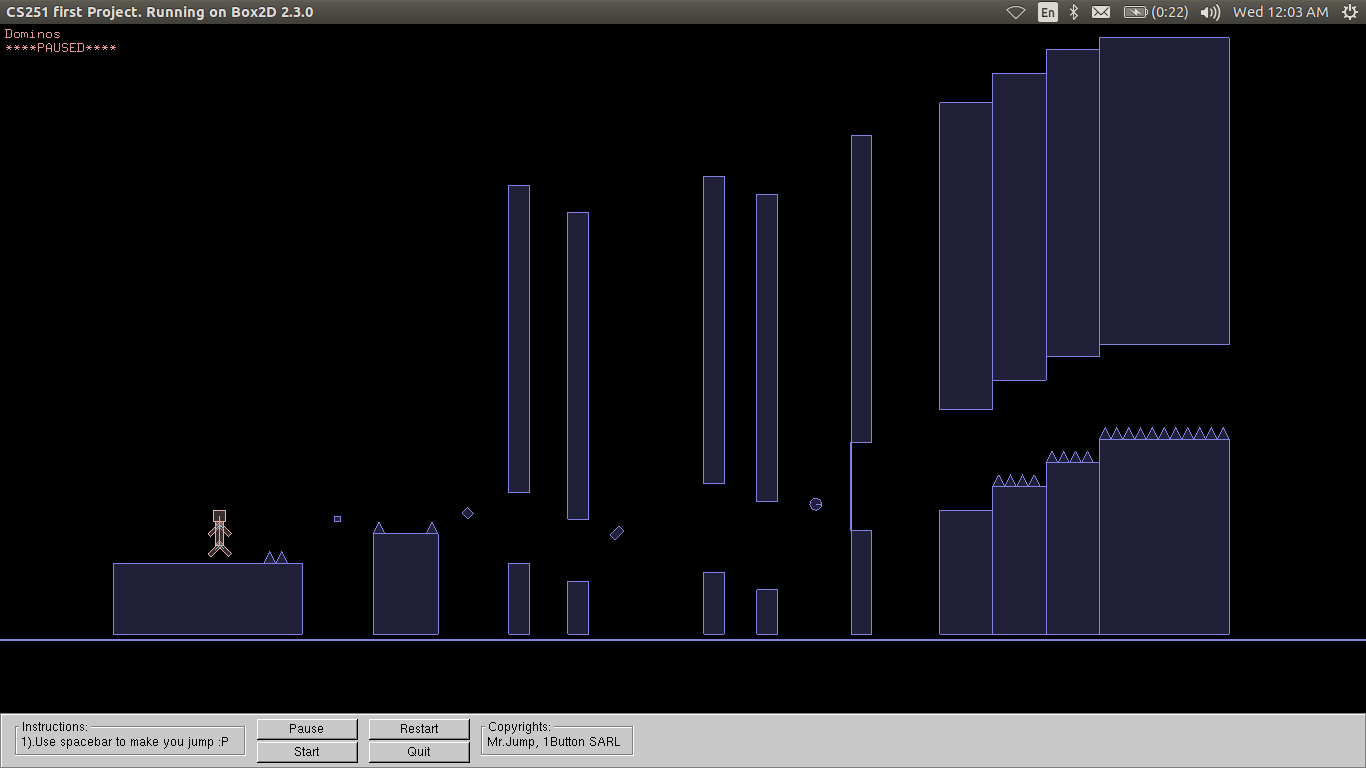
\includegraphics[width=6in]{Box2D}
\caption{A screenshot of final game.}
\label{fig:1}
\end{figure}
\section{Description on final game}
\paragraph{Description:}
{\bf There are atleast 10 elements in this game.There is a man who is the player of the game.There are triangle shaped obstrucles which when touched by the man ends the game.Then there is ground, below which there is water which ends the game if the man falls into it.There are many powerups in the game.One powerup in rhombus shape gives a instantaneous jump.Another one in rectangle shape gives infinite jumps.The circular one opens the corresponding door which makes them two more elements.There is also a rocket powerup which when gained gives upward velocity as long as the key is pressed until it touches the ground.}

\newpage
\section{Project Details}

\subsection{TITLE}
{\bf Jumping Stick Man}\\

\subsection{Motivation}
We want to build a game which resembles nearly to the present android games which are growing a lot these days.

\subsection{Project Goal}
\paragraph{}
 We are hoping to build a small Box2D game similar to the Mr.Jump game in itunes \cite{WinNT}.\\It consists a minimum of 10 elements as part of the game and we will decide the levels according to the time available for us.It is basically a typical game in which the player has to move front without hitting any obstrucles and has some power elements as he passes through the game.

\subsection{Achievement}
\paragraph{}
 We were able to build the game engine with all the components in it as per our design.The game runs sufficiently good with some minor bugs in the termination condition like when the game should end.

\subsection{Failures}
\paragraph{}
 We could not implement water in the game.So we just created an edge in place of water.There is one bug left out that is too difficult for us to understand as they are problems from the libraries in the operating system.

\subsection{Work-Done}
\paragraph{}
Nihal:
 1)Created the man in the game.\\
 2)worked on contactlistner callbacks\\
 3)coded for powerups\\
 3)made vedio and documentation comments\\

Lohith:\\
 1)Created all the remaining bodies.\\
 2)worked on contactlistner callbacks\\
 3)coded for gameover conditions\\
 4)made report and finalising submission\\

 Jagadeesh:\\
 1)worked on debugging the code.\\
 2)profiling the code.\\
 3)created the html page.\\

\subsection{Difficulties}
1)Taking input and making the man jump was the first difficulty faced.\\
2)we could do it by reading the box2d tutorials.\\
3)The second difficulty was detecting the contact.\\
4)we din't use m\_world->SetContactListner(this); in the constructor of the class in which we were using the contactlistner function.\\
5)we corrected it after suggestion from Sahith Thallapally.\\
6)The next difficulty was differentiating powerups and the conditions for gameover.\\
7)Nihal worked on powerups.\\
8)lohith worked on gameover conditions.\\
9)we tried to use the userdatafunction to store an integer and differentiating the bodies.\\
10)we had problem that the return value of getuserdata function which is of the type Void* is getting optimized out.\\
11)We created two new functions called GetIntValue and SetIntValue inside the box2d folder in cs251\_base\_code/external/src/Box2d/Box2d/Dynamics/Box2d.h,Box2d.cpp.\\
12)We used these functions to differentiate the bodies.\\
13)Nihal used enum function to get the powerup powers.\\

\subsection{Profile}
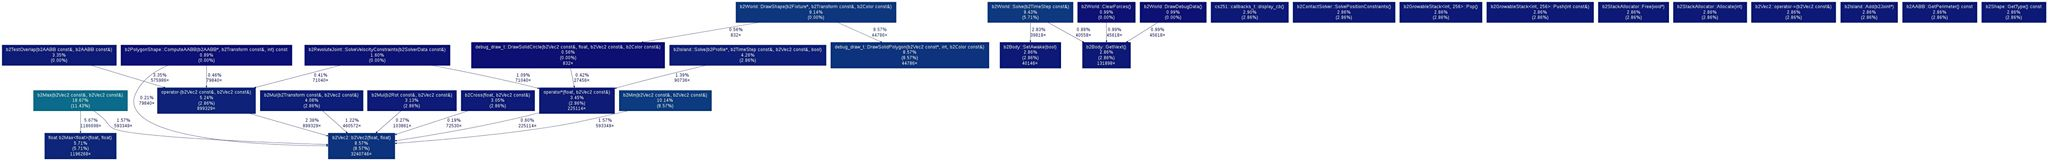
\includegraphics[width=6in]{profile}
\subsection{Help from previous labs}
1) We were able to find that the return value of getuserdata is getting optimized out using gdb debugging.\\
\bibliography{Projectreport}
\bibliographystyle{plain}
\end{document}
